\documentclass[letterpaper,12pt,oneside]{article}\usepackage[]{graphicx}\usepackage[]{color}
%% maxwidth is the original width if it is less than linewidth
%% otherwise use linewidth (to make sure the graphics do not exceed the margin)
\makeatletter
\def\maxwidth{ %
  \ifdim\Gin@nat@width>\linewidth
    \linewidth
  \else
    \Gin@nat@width
  \fi
}
\makeatother

\definecolor{fgcolor}{rgb}{0.345, 0.345, 0.345}
\newcommand{\hlnum}[1]{\textcolor[rgb]{0.686,0.059,0.569}{#1}}%
\newcommand{\hlstr}[1]{\textcolor[rgb]{0.192,0.494,0.8}{#1}}%
\newcommand{\hlcom}[1]{\textcolor[rgb]{0.678,0.584,0.686}{\textit{#1}}}%
\newcommand{\hlopt}[1]{\textcolor[rgb]{0,0,0}{#1}}%
\newcommand{\hlstd}[1]{\textcolor[rgb]{0.345,0.345,0.345}{#1}}%
\newcommand{\hlkwa}[1]{\textcolor[rgb]{0.161,0.373,0.58}{\textbf{#1}}}%
\newcommand{\hlkwb}[1]{\textcolor[rgb]{0.69,0.353,0.396}{#1}}%
\newcommand{\hlkwc}[1]{\textcolor[rgb]{0.333,0.667,0.333}{#1}}%
\newcommand{\hlkwd}[1]{\textcolor[rgb]{0.737,0.353,0.396}{\textbf{#1}}}%

\usepackage{framed}
\makeatletter
\newenvironment{kframe}{%
 \def\at@end@of@kframe{}%
 \ifinner\ifhmode%
  \def\at@end@of@kframe{\end{minipage}}%
  \begin{minipage}{\columnwidth}%
 \fi\fi%
 \def\FrameCommand##1{\hskip\@totalleftmargin \hskip-\fboxsep
 \colorbox{shadecolor}{##1}\hskip-\fboxsep
     % There is no \\@totalrightmargin, so:
     \hskip-\linewidth \hskip-\@totalleftmargin \hskip\columnwidth}%
 \MakeFramed {\advance\hsize-\width
   \@totalleftmargin\z@ \linewidth\hsize
   \@setminipage}}%
 {\par\unskip\endMakeFramed%
 \at@end@of@kframe}
\makeatother

\definecolor{shadecolor}{rgb}{.97, .97, .97}
\definecolor{messagecolor}{rgb}{0, 0, 0}
\definecolor{warningcolor}{rgb}{1, 0, 1}
\definecolor{errorcolor}{rgb}{1, 0, 0}
\newenvironment{knitrout}{}{} % an empty environment to be redefined in TeX

\usepackage{alltt}
\usepackage[paperwidth=8.5in,paperheight=11in,top=1in,bottom=1in,left=1in,right=1in]{geometry}
\usepackage{setspace}
\usepackage[colorlinks=true,allcolors=Blue]{hyperref}
\usepackage[usenames,dvipsnames]{xcolor}
\usepackage{indentfirst}
\usepackage{titlesec}
\usepackage{multirow}
\usepackage{booktabs}
\usepackage{graphicx}
\usepackage{verbatim}
\usepackage{rotating}
\usepackage{tabularx}
\usepackage{outlines}
\usepackage{lineno}
\usepackage{array}
\usepackage{times}
\usepackage{cleveref}
\usepackage{acronym}
\usepackage[position=t]{subfig}
\usepackage{paralist}
\usepackage[noae]{Sweave}
\usepackage{natbib}
\usepackage{array}
\usepackage{pdflscape}
\usepackage{bm}
\usepackage{showlabels}
\bibpunct{(}{)}{,}{a}{}{,}

% page margins and section title formatting
\linespread{2}
\setlength{\footskip}{0.5in}
\titleformat*{\section}{\Large\bf\em}
\titleformat*{\subsection}{\singlespace\large\bf}
\titleformat*{\subsubsection}{\singlespace\normalsize\bf\em}
\titlespacing{\section}{0in}{0in}{0in}
\titlespacing{\subsection}{0in}{0in}{0in}
\titlespacing{\subsubsection}{0in}{0in}{0in}

% cleveref options
\crefname{table}{Table}{Tables}
\crefname{figure}{Fig.}{Figs.}
\renewcommand{\figurename}{Fig.}

% aliased citations
\defcitealias{CDMO14}{CDMO 2014}
\defcitealias{RDCT14}{RDCT 2014}

% acronyms
\acrodef{DO}[DO]{dissolved oxygen}
\acrodef{NERRS}[NERRS]{National Estuarine Research Reserve System}
\acrodef{RMSE}[RMSE]{root mean square error}
\acrodef{SWMP}[SWMP]{System Wide Monitoring Program}
\acrodef{WRTDS}[WRTDS]{weighted regression on time, discharge, and season}

% assorted functions
% for multiple rows in table headers
\newcommand{\head}[2]{\multicolumn{1}{>{\arraybackslash}p{#1}}{#2}}
% for milligrams per litre
\newcommand{\mgl}{mg L$^{-1}$}

% hides (not removes) numbering for section, subsection, etc.
% left indents
\renewcommand{\thesection}{}
\renewcommand{\thesubsection}{}
\renewcommand{\thesubsubsection}{}
\makeatletter
\def\@seccntformat#1{\csname #1ignore\expandafter\endcsname\csname the#1\endcsname\quad}
\let\sectionignore\@gobbletwo
\def\@subseccntformat#1{\csname #1ignore\expandafter\endcsname\csname the#1\endcsname\quad}
\let\subsectionignore\@gobbletwo
\def\@subsubseccntformat#1{\csname #1ignore\expandafter\endcsname\csname the#1\endcsname\quad}
\let\subsubsectionignore\@gobbletwo
\let\latex@numberline\numberline
\def\numberline#1{\if\relax#1\relax\else\latex@numberline{#1}\fi}
\makeatother

%knitr options


% dependent data



\IfFileExists{upquote.sty}{\usepackage{upquote}}{}
\begin{document}

\raggedbottom
% \linenumbers
\raggedright
\urlstyle{same}
\setlength{\parindent}{0.5in}
\renewcommand\refname{References \vspace{12pt}}

%%%%%%
% title page
\begin{singlespace}
\title{{\bf {\Large Improving estimates of ecosystem metabolism by removing effects of tidal advection in dissolved oxygen time series}}}
\author{
  {\bf {\normalsize Marcus W. Beck$^1$, Michael C. Murrell$^2$, James D. Hagy III$^2$}}
  \\\\{\textit {\normalsize $^1$ORISE Research Participation Program}}
  \\{\textit {\normalsize USEPA National Health and Environmental Effects Research Laboratory}}
	\\{\textit {\normalsize Gulf Ecology Division, 1 Sabine Island Drive, Gulf Breeze, FL 32561}}
	\\{\textit {\normalsize Phone: 850-934-2480, Fax: 850-934-2401, Email: \href{mailto:beck.marcus@epa.gov}{beck.marcus@epa.gov}}}
  \\\\{\textit {\normalsize $^2$USEPA National Health and Environmental Effects Research Laboratory}}
	\\{\textit {\normalsize Gulf Ecology Division, 1 Sabine Island Drive, Gulf Breeze, FL 32561}}
	\\{\textit {\normalsize Phone: 850-934-2433, Fax: 850-934-2401, Email: \href{mailto:murrell.michael@epa.gov}{murrell.michael@epa.gov}}}
  \\\\{\textit {\normalsize $^3$USEPA National Health and Environmental Effects Research Laboratory}}
	\\{\textit {\normalsize Gulf Ecology Division, 1 Sabine Island Drive, Gulf Breeze, FL 32561}}
	\\{\textit {\normalsize Phone: 850-934-2455, Fax: 850-934-2401, Email: \href{mailto:hagy.jim@epa.gov}{hagy.jim@epa.gov}}}
	}
\date{}
\maketitle
\vfill{\centerline{\textit {\normalsize Running head: Improving Estimates of Estuary Metabolism}}}
\end{singlespace}
\clearpage

%%%%%%
% acknowledgments
\section{Acknowledgments}

%%%%%%
% abstract
\centerline{{\bf Abstract}}
\begin{singlespace} \small
\noindent 
Reliable estimates of ecosystem metabolism depend on measures of \ac{DO} flux that are dominated by biological processes.  Long-term time series of \ac{DO} measurements may include variation related to both biological and physical processses such that the use of observed data may be insufficient or even misleading in some examples.  Statistical modelling techniques that dynamically quantify variation in \ac{DO} over time and tidal changes have the potential to isolate biological signals in \ac{DO} variation to more accurately estimate metabolism.  A weighted regression method that estimates \ac{DO} as a function of time and tidal height was developed to normalize, or detide, the predicted \ac{DO} signal to remove the influence of physical advection on metabolism estimates.  First, a simulation approach was used to create multiple \ac{DO} time series with known additive components of biological and physical variation on different periods.  Comparisons of detided estimates with the known, simulated biological component of the \ac{DO} signal suggested the method accurately and precisely removed varation attributed to tidal advection.  Extension of the method to four case studies provided a proof of concept illustrating the method could be useful for real-world applications. We provide a detailed discussion on use of the method for improving certainty in evaluation of \ac{DO} measurements from sites with strong tidal influences.  Moreover, we propose that the method could expand use of the open-water method for estimating ecosystem metaoblism in estuaries given that the approach can produce robust estimates of \ac{DO} values that are independent of tidal advection.  In particular, this could facilitate the use of shorter deployment periods for water quality monitors or incomplete time series given that known biases related to water movement could be removed with weighted regression. 
\normalsize
\end{singlespace}
\noindent {\bf Key words}:

\acresetall
\clearpage

%%%%%%
% intro
\section{Introduction} \label{intro}

Ecosystem metabolism is broadly defined as the difference between primary production and aerobic respiration and provides a basis for evaluating trophic state \citep{Kemp12,Needoba12}.  Primary producers, such as phytoplankton, establish the means of energy transfer to upper trophic levels. Productive systems are characterized by more efficient transfer of organic matter between trophic levels, whereas less productive systems are sinks of organic matter that are supported by allochthonous sources of energy input.  The balance between production and respiration is an integrated measure of metabolism that accounts for varying rates in processes that create and consume organic matter.  Although metabolic rates vary naturally in different regions \citep{Caffrey04}, human activities and infrastructure development are contributing factors that increase rates of production \citep{Diaz08}.  Inputs of limiting nutrients beyond background concentrations may decrease the resilience of an ecosystem such that higher rates of production are coupled with higher biological oxygen demand \citep{Yin04,Kemp09}.  Cultural eutrophication is frequently linked to declines in water quality through lower levels of dissolved oxygen and increased frequency of noxious algal blooms.  Reliables estimates of ecosystem metabolism are critical for measuring both background rates of production and potential impacts of human activities on ecosytem condition.     

Ecosystem metabolism can be estimated using several techniques, each of which is appropriate under different conditions or assumptions.   Bottle-based techniques rely on rate measurements from discrete water quality samples, whereas open-water techniques infer metabolic rates using \textit{in situ} measurements from continuous monitoring data.  Bottle-based techniques are useful for direct partitioning of metabolic contributions into discrete habitats, such as planktonic production rates during specific time periods \citep{Kemp12}.  However, such measurements may be inappropriate for evaluating whole ecosystem metabolism if significant production occurs in habitats that are not sampled, such as benthic or seagrass production.  As such, the open-water technique provides an integrative measure of metabolism by inferring process rates from \textit{in situ}, continuous monitoring data.  Originally proposed for use in streams \citep{Odum56}, the method has been used with varying success in lakes \citep{Staehr10,Coloso11,Batt12} and estuaries \citep{Caffrey04,Hopkinson05,Caffrey13}.  The ability of the open-water method to accurately estimate metabolism depends on whether the assumptions for its use are met, which are often only implicity verified in practiced. 

The open-water method uses the diel fluctuation of dissolved oxygen to infer rates of ecosytem metabolism, after correcting for losses or gains through air-water exchange \citep{Kemp12}.  Daily integrated measurements of metabolism are based on the balance between daytime estimates of gross production and nighttime estimates of respiration extrapolated to a 24 hour period.  The fundamental assumption of the open-water method is that measurements come from a water mass that has the same recent history \citep{Needoba12}.  Estimates of metabolism from a single location may be inaccurate if substantial variation in water column mixing occurs throughout the period of observation.  As such, the original technique designed for use in streams requires the comparison of data from an upstream and downstream station \citep{Odum56}.  Application of the method to systems without continuous flow, such as lakes or estuaries, have often assumed that a single sampling station provides sufficient data for estimating metabolism \cite{Staehr10}.  While single stations may be valid under specific conditions, numerous studies have shown that the open-water method may be inappropriate given the effects of physical mixing \citep{Ziegler98,Caffrey03,Coloso11,Batt12,Nidzieko14}.

The open-water method has recently been applied to coastal and oceanic ecosystems with mixed success.  An exhaustive analysis by \citet{Caffrey03} applied the method to estimate metabolim at 28 continuous monitoring stations at 14 US estuaries.  Data from two of the reserves were used to evaluate the assumption of homogeneity of water masses measured by each sensor.  Although significant differences were not observed for metabolism estimates between adjacent stations, the analysis was based on a comparison of means using conventional significance tests rather than a systematic comparison of time series.  Moreover, a portion of metabolism estimates from all stations were negative for production during the day and positive for respiration during the night.  These values were opposite in sign than expected since production increases oxygen during the day (i.e., positive effect on metabolism) and respiration consumes oxygen at night (i.e., negative effect on metabolism).  These `anamolous' values were attributed to violations in the assumption of water-column heterogeneity.  Specifically, tidal variation could have caused sampling of different water masses by individual water quality sondes as water moved inland or seaward with changing tide. 

The effects of tidal advection on estimates of ecosystem metabolism have been a point of concern in numerous studies \citep{Ziegler98,Caffrey03,Collins13,Howarth14}, although systematic estimates of its effects and methods for accounting for physical variation in \ac{DO} measurements have been minimal.  An exception is presented by \citet{Nidzieko14} through quantitative assessment of the effects of fortnightly tidal modulations on metabolism estimates.  Using a control volume approach to measure fluxes into and out of a shallow tidal creek, significant biases in metabolism estimates were observed.  Net heterotrophy was observed during spring tides, whereas metabolism was balanced during neap tides.  The timing of irradiance relative to the tidal cycle was a primary factor contributing to heterotrophy during summer months such that maximum tides occurred during the night, increasing total area for respiration.  The results of the analysis, although specific to the study location, suggest that the effects of tidal advection on \ac{DO} measurements are of primary concern when selecting locations and length of time for sonde deployment in estuaries.  In many cases, the relative magnitude of these effects may be a significant source of bias without quantitative evaluation to determine the roles of biological and physical signals in \ac{DO} measurements. Analytical techniques to evaluate and correct for tidal advection could improve certainty in metabolism estimates and also increase the use of data from shorter deployment periods if sources of bias are quantified and removed.       

This article describes use of a novel method for quantifying and removing noise in estimates of ecosystem metabolim for estuaries.  Specifically, we characterize the effects of tidal advection on \ac{DO} observations to improve estimates of open-water metabolism with multi-year time series of high frequency ($<$ one hour) water quality data.  The focus of our analysis is the use of a weighted regression method previously developed for trend analysis of pollutant concentrations in streams and rivers \citep{Hirsch10}.  A weighted regression approach is applied to create dynamic predictions of \ac{DO} as a function of time and tidal height change, which is then used to normalize, or detide, the \ac{DO} signal.  The analysis is presented in two steps.  First, we apply a simulation approach to create time series of \ac{DO} observations with known characteristics to evaluate ability of the weighted regression to predict the time series and remove the effects of tidal advection.  Second, four case studies of multi-year time series are used to further explore use of the weighted regression approach to remove potential noise in \ac{DO} signals from tidal advection.  Comparisons of observed and detided \ac{DO} values are compared, in addition to estimates of open-water metabolism before and after detiding of the \ac{DO} time series.  Overall, the analysis provides a means to improve certainty in conclusions from observed \ac{DO} for evaluating the relative roles of biological and physical processes in estuarine systems.  Applications of the weighted regression approach are expected to have wide-ranging implications for management and ecosystem monitoring by outlining strategies for obtaining water quality estimates with more accuracy.

%%%%%%
% materials and procedures
\section{Materials and Procedures}

\subsection{Weighted regression for modelling and detiding \ac{DO} time series}

The weighted regression model for detiding \ac{DO} time series was adapted from the \ac{WRTDS} method developed by \citet{Hirsch10}.  The \ac{WRTDS} method was developed to model pollutant concentration in streams and normalize predictions to changes in discharge.  The functional form of our model is as follows:
\begin{equation}\label{funform}
DO_{obs}= \beta_0 + \beta_1 t + \beta_2 H
\end{equation}
where observed \ac{DO} is a linear function of decimal time $t$ and astronomical tidal height $H$. Decimal time is a continuous variable for the day and time of each obervation with time as a proportion of the number of total observations added to each day.  The beginning of each day was considered the nearest thirty minute observation (i.e., on the hour and half hour) at which sunrise was expected for a given location and time of year.  Days were centered on the diel cycle rather than conventional times given that the objective was to develop a predictive model relevant for biological \ac{DO} variation that follows solar and seasonal cycles.  The functional form also differed from the original \ac{WRTDS} method that included parameters to estimate variation of the response variable on a sinuisoidal period.  \ac{DO} variation was not modeled using this approach because rates of change may be abrupt following diurnal variation in irradiance or daily \ac{DO} variation may be muted given the weather, as on cloudy days.

Weighted regression is implemented as a moving window that allows for estimation of \ac{DO} throughout the time series by adapting to variation through time as a function of tide. Regression models are estimated sequentially for each observation in the time series using dynamic weight vectors that change with the center of the window.  Weight vectors quantify the relevance of observations to the center of the window in respect to decimal time, hour of the day, and tidal height.  Specifically, weights are assigned using a tri-cube weighting function \citep{Hirsch10}:
\begin{equation}
w= \left\{ 
  \begin{array}{l l}
    \left(1-\left(d/h\right)^3\right)^3 & \quad \textrm{if } |d| \leq h \\
    0 & \quad \textrm{if } |d| > h 
  \end{array} \right.
\end{equation}
where the weight $w$ of each observation is inversely proportional to the distance $d$ from the center of the window such that observations more similar to the point of reference are given higher importance in the regression.  Weights exceeding the maximum width of the window $h$ are equal to zero.  The tri-cube weighting function is similar to a normal distribution such that weights decrease gradually from the center until the maximum window width is reached.  Observations that are half the distance from the center of the window to the maximum window width are weighted 1/3 less than values at the center.  Regressions that use simpler windows (e.g., boxcar approach) are  more sensitive to influential observations as they enter or leave the window, whereas the tri-cube function minimizes their effect through gradual weighting of observations \citep{Hirsch10}.  The weight vector for each observation is the product of three separate weight vectors for decimal time, hour, and tidal height. A low weight is given to an observation if any of the three weighting values were not similar to the center of the window since the final weight vector is the product of three weight vectors for each variable.    

A nontrivial issue with weighted regression is the choice of window width for calculating weights.  Excessively large or small window widths may respectively under- or over-fit the data.  Additionally, optimal window widths may depend on the objective for using the model.  The weighted regression approach can be used for both predicting \ac{DO} and normalizing to remove the variance in the \ac{DO} signal from tidal changes.  Optimal window widths that minimize prediction error or fit to the observed data are typically smaller than the optimum window widths for normalizing the time series.  Similarly, window widths that more effectively detide the \ac{DO} signal may produce predictions for the observed data that are not optimal.  Evaluations of the weighted regression method with simulated \ac{DO} time series, described below, used different window widths to identify an approximate optimal window width for detiding the \ac{DO} signal.  As such, the ability of the models to predict observed \ac{DO} was not a primary concern given that the optimal window width for detiding likely corresponds to a model that predicts \ac{DO} as a function of tide rather than observed \ac{DO} as a function of both tide and biological variation.  

\subsection{Detiding the \ac{DO} signal using weighted regression}

The primary objective of the analysis was to evaluate ability of the weighted regression method to detide a \ac{DO} signal to obtain more accurate estimates of metabolism.  \citet{Hirsch10} developed the normalization approach for the \ac{WRTDS} method using a two-dimensional interpolation grid that contains predicted values of pollutant concentrations across the time series and the range of stream discharge values observed in the study system \citep{Hirsch10}.  Normalized values for pollutant concentration are obtained by averaging the model predictions across the discharge values that are likely to occur on a given day to provide an estimate that is independent of flow variation.    

Predicted values of \ac{DO} concentration were normalized to remove variation from tidal height changes, although the approach herein differs slightly from \citet{Hirsch10}.  Our approach uses weighted regression to isolate sources of variation in the observed \ac{DO} signal that are related to unique effects of tidal height and biological process (\cref{fig:do_dtd}).  Two sets of values are predicted for the observed time series $DO_{obs}$, rather than creating an interpolation grid.  The first set of values uses the tidal height of an observation and second set uses the mean tidal height across the time series, $DO_{tid}$ and $DO_{nrm}$ respectively.  In other words, the first set of predictions represent \ac{DO} as a function of time and tide, where the second set represents \ac{DO} conditional on time and mean tidal height:
\begin{equation} \label{do_tid}
DO_{tid} = f(DO_{obs}|H, t)
\end{equation}
\begin{equation} \label{do_nrm}
DO_{nrm} = f(DO_{obs}|\bar{H}, t)
\end{equation}

%%%%%%
% assessment
\section{Assessment}

\subsection{Simulation of \ac{DO} time series}

The ability of the weighted regression to detide the \ac{DO} signal was evaluated first using a simulation approach.  Observed \ac{DO} time series were created to represent the sum of variation from biological processes and physical effects related to tidal advection:  
\begin{equation} \label{do_obs}
DO_{obs} = DO_{bio} + DO_{adv}
\end{equation}
Biological \ac{DO} signals are inherently noisy \citep{Batt12} and can be further described as:
\begin{equation} \label{do_bio} 
DO_{bio} = DO_{die} + DO_{unc}
\end{equation} 
\begin{equation} \label{do_unc}
DO_{unc} = \epsilon_{obs} + \epsilon_{proc}
\end{equation}
where the biological \ac{DO} signal is the sum of diel variation on a 24 hour scale plus uncertainty or noise.  Total uncertainty in the biological \ac{DO} signal is described as variation from observation and process uncertainty \citep{Hilborn97}.  Multiple time series at 30 minute observations over 30 days were created following \cref{do_obs,do_bio,do_unc} such that observed \ac{DO} is generalized as the additive combination of four time series (\cref{fig:do_sim}):
\begin{equation} \label{do_obs_all}
DO_{obs} = DO_{adv} + DO_{die} + \epsilon_{obs} + \epsilon_{pro}
\end{equation}
Time series were created by varying the relative magnitudes of each of the four components of observed \ac{DO} to test the effectiveness of weighted regression under different scenarios.  The effects of air-sea gas exchange were not considered in the simulation given that methods are available for \textit{in situ} data to correct observed \ac{DO} for diffusion \citep[i.e., ][]{Thebault08}.  

Each parameter of the simulated time series was created as follows. First, biological \ac{DO} time series in \cref{do_bio} were created by adding noise or variance to a diel component (\cref{fig:do_sim}).  The diel component, $DO_{die}$, was estimated using a sine/cosine function \citep{Cryer08}:
\begin{equation} \label{do_sin}
DO_{die} = \alpha + \beta\cos\left(2\pi ft + \Phi\right)
\end{equation}
such that the mean DO $\alpha$ was 8, amplitude $\beta$ was 1, $f$ was 1/48 to repeat on a 24 hour period every 30 minutes, $t$ was the time series vector and $\Phi$ was the x-axis origin set for an arbitrary sunrise at 630am.  The diel signal was increasing during the day and decreasing during the night for each 24 hour period and ranged from 7 to 9 mg L$^{-1}$.  Noise or uncertainty was added to the diel \ac{DO} signal to simulate natural variation in \ac{DO} throughout the time series (\cref{fig:do_sim}).  Total uncertainty was the sum of observation and process uncertainty for $n = 1440$ (30 minutes by 30 days) observations \citep{Hilborn97}, such that:
\begin{equation} \label{do_unc_n}
DO_{unc, n} = \epsilon_{obs, n} + \int_{t = 1}^{n} \epsilon_{pro, t}
\end{equation}
where observation and process uncertainty ($\epsilon_{obs}$, $\epsilon_{pro}$) were simulated as normally distributed random variables with mean zero and standard deviation varying from zero to an upper limit, described below.  To induce auto-correlation, process uncertainty was estimated as the cumulative sum of $n$ observations where the noise at time $t+1$ was equal to the noise at time $t$ plus additional variation drawn from the normal distribution.  The noise vector for process uncertainty was rescaled to constrain the variation within the bounds for standard deviation defined by the random variable. The total uncertainty, $DO_{unc}$, was added to the diel \ac{DO} time series to create the biological \ac{DO} time series (\cref{fig:do_sim}).

A tidal time series was simulated by adding sine waves (harmonics) with relevant solar and lunar periods \citep{Foreman89}.  Each sine wave was created using \cref{do_sin} by varying $f$ for periods that approximated common tidal components, e.g., 1/25 for a 12.5 hour principal lunar semi-diurnal wave.  The amplitude of each tidal component was set constant to one meter.  The combined tidal series was the additive time series of all sine waves, scaled to 1 meter and centered  at 4 meters.  The tidal time series was added to the biological \ac{DO} series to simulate \ac{DO} changes with advection, $DO_{adv}$ (\cref{fig:do_sim}). Conceptually, this vector represents the rate of change in \ac{DO} as a function of horizontal water movement from tidal advection such that:
\begin{equation} \label{deltdo}
\frac{\delta DO_{adv}}{\delta t} = \frac{\delta DO}{\delta x} \cdot \frac{\delta x}{\delta t}
\end{equation}
\begin{equation} \label{deltx}
\frac{\delta x}{\delta t} = k \cdot \frac{\delta H}{\delta t}
\end{equation}
where the first derivative of the tidal time series, as change in height over time $\delta H / \delta t$, is multiplied by a constant $k$, to estimate horizontal tidal excursion over time, $\delta x / \delta t$.  The horizontal excursion is assumed to be associated with a horizontal \ac{DO} change, $\delta DO / \delta x$, such that the product of the two estimates the \ac{DO} change at each time step from advection, $DO_{adv}$. In practice, the simulated tidal signal was used to estimate $DO_{adv}$:
\begin{equation} \label{do_advp}
DO_{adv} \propto H
\end{equation}
\begin{equation} \label{do_adv}
DO_{adv} = 2\cdot a + a \cdot \frac{H- \min H}{\max H - \min H}
\end{equation}
where $a$ is analogous to $k$ in \cref{deltx} and is chosen as the transformation parameter to standardize change in \ac{DO} from tidal height change to desired units.  For example, $a = 1$ will convert $H$ to a scale that simulates changes in \ac{DO} from tidal advection that range from +/- 1 mg L$^{-1}$.  The final time series for observed \ac{DO} was the sum of biological \ac{DO} and advection \ac{DO} (\cref{fig:do_sim}).

\subsection{Evaluation of weighted regression with simulated \ac{DO} time series}

Multiple time series were simulated by varying the conditions in \cref{do_obs,do_bio,do_unc,do_obs_all,do_sin,do_unc_n,deltdo,deltx,do_advp,do_adv}. Specifically, the simulated data varied in the relative amount of noise in the measurement, relative amplitude of the diel \ac{DO} component, degree of association of the tide with the \ac{DO} signal, and tidal type as diurnal, semidiurnal, and mixed semidiurnal.  Three levels were evaluated for each variable: relative noise as 0, 1, and 2 standard deviations for both process and observation uncertainty, amplitude of diel biological \ac{DO} as 0, 1, and 2 mg L$^{-1}$, and \ac{DO} change from tidal advection as 0, 1, and 2 mg L$^{-1}$.  Three tidal categories were created from \cref{do_sin} using a period of 24.82 hours (principal lunar) for diurnal, 12.42 hours (principal lunar semidiurnal) for semidiurnal, and adding both diurnal and semidiurnal series for mixed semidiurnal. A total of 243 time series were created based on 81 unique combinations of parameters for each tidal category (\cref{fig:sim_ex}).  Three window widths for each variable used to estimate the total weight vector were evaluated (as half window widths): decimal time as 1, 3, and 8 days, time of day as 6, 12, and 24 hours, and tidal height as 0.25, 0.5, and 1 as a proportion of the observed value at the center of the window.  In total, 27 window width combinations were evaluated for each of 243 simulated time series, producing results for 6561 weighted regressions.

The detided or normalized values for each regression were compared to the simulated data to evaluate the ability of weighted regression to reproduce the biological \ac{DO} signals. Results were summarized using Pearson correlation coefficients and the \ac{RMSE} between the predicted and observed \ac{DO} values and the detided and biological \ac{DO} values.  Overall, the weighted regressions provided accurate results for the detided time series compared to the `true' biological time series regardless of the simulation parameters (\cref{tab:dtd_perf1}) or window widths (\cref{tab:dtd_perf2}).  Mean correlation for all time series and window widths between the detided and biological values was 0.56, with values ranging from -0.78 to 1.00.  Mean error was 1.27, with values ranging from 0.00 to 2.47.  Simulations with very poor performance (e.g., negative correlations) were those that had minimum widths for day windows and maximum widths for hour windows, or were those with the \ac{DO} signal composed entirely of noise from observation uncertainty. Conversely, simulations with detided time series that were identical to the true time series (e.g., correlation of one, \ac{RMSE} of zero) were those for which there was no biological or tidal influence.  While the latter examples do not represent real-world scenarios, they were included in the simulations to provide verification that the weighted regressoin provide reasonable results in extreme scenarios.  

Characteristics of \ac{DO} time series that contributed to improved model performance were increasing amplitude of the diel \ac{DO} component ($DO_{die}$) and increasing process uncertainty ($e_{pro}$), whereas increasing observation uncertainty contributed to decreasing performance (\cref{tab:dtd_perf1}).  Model performance was minimally influenced by magnitude of the tidal advection component ($DO_{adv}$), although performance decreased slightly with increasing tidal effects.  Increasing widths for day and tidal proportion windows contributed to increasing model performance, whereas the opposite was true for increasing hour windows (\cref{tab:dtd_perf2}).  Graphical summaries of model performance by simulation parameters (\cref{fig:err_surf1}) and half window widths (\cref{fig:err_surf2}) supports the general trends described by \cref{tab:dtd_perf1,tab:dtd_perf2}.  Scale differences between \cref{fig:err_surf1} and \cref{fig:err_surf2} emphasize that model performance was more affected by characteristics of the \ac{DO} time series rather than the selected window widths.  For example, the range of correlation values comparing the effects of half window widths (averaged across all simulation parameters, \cref{fig:err_surf2}) were approximately half the range of correlations for comparing the effects of simulation parameters (averaged across all half window widths, \cref{fig:err_surf1}).
 
\subsection{Validation of weighted regression with case studies}

The \ac{NERRS} is a federally-funded network of 28 protected estuaries established for long-term research, water-quality monitoring, education, and coastal stewardship \citep{Wenner04}.  Continuous water quality data have been collected at \ac{NERRS} sites since 1994 through the \ac{SWMP}.  In addition to providing a basis for trend evaluation, data from \ac{SWMP} provides an ideal opportunity to evaluate long-term variation in water quality parameters attributed to both biological and physical processes.  Continuous \ac{SWMP} data can be used to describe \ac{DO} variation at sites with different characteristics, including variation from ranges in tidal regime \citep{Sanger02} and rates of ecosystem production \citep{Caffrey03,Caffrey04}.  

Continuous \ac{DO} time series and tidal height measurements at four sites from the \ac{SWMP} database \citepalias{CDMO14} were used to further validate the weighted regression model.  Monitoring data from January 1\textsuperscript{st} to December 31\textsuperscript{st} 2012 were obtained from a range of geographic locations (\cref{fig:case_map,tab:case_att}). Astronomical tidal heights were predicted for each site using harmonic regression applied to the sonde depth data (\texttt{oce} package in R, \citealt{Foreman89}, \citetalias{RDCT14}). Although, the depth data represent tidal height variation from both astronomical (i.e., gravitational effects) and meteorological (e.g., wind, precipitation inflows) sources, we isolated the former given that daily metabolism estimates were more likely to be affected by repeated diel cycling from normal tidal changes.  Each station was also chosen based on high correlations between \ac{DO} and tidal changes.  The four sites included the Vierra Mouth station at Elkhorn Slough (California, 36.81$^{\circ}$N, 121.78$^{\circ}$W), Bayview Channel at Padilla Bay (Washington, 48.50$^{\circ}$N 122.50$^{\circ}$W), Middle Blackwater River station at Rookery Bay (Florida, 25.93$^{\circ}$N 81.60$^{\circ}$W), and Dean Creek station at Sapelo Island (Georgia, 31.39$^{\circ}$N 81.28$^{\circ}$W).  The stations are generally macrotidal semidiurnal or mixed semidiurnal and net heterotrophic on an annual basis.  Net heterotrophy (i.e., respiration exceeding production) is typical for shallow water systems at temperate latitudes \citep{Caffrey03}, although values in \cref{tab:case_att} are from observed \ac{DO} time series that are strongly influenced by tidal advection.

\subsection{Estimates of ecosystem metabolism before and after detiding}

The weighted regression method was applied to the time series for each station to obtain a detided \ac{DO} time series for estimating metabolism.  The half window widths that produced the most robust results for the simulations were used for the case studies: eight days, six hours, and a tidal proportion of one. Unlike the simulated data, the true biological \ac{DO} signal was unknown for the case studies.  Accordingly, results were evaluated  using correlations of \ac{DO} and metabolism estimates with tidal height before and after application of the model.  Results were also evaluated based on the occurrence of `anomalous' daily production or respiration estimates, where anomalous was defined as negative production during the day and positive respiration estimates during the night.  Anomalous values have been previously attributed to the effects of physical processes on \ac{DO} time series \citep{Caffrey03}.  We hypothesized that metabolism esimates using the detided signal would contain less `anomalous' values than those from the observed \ac{DO} time series.  Although anomalies could be caused by processes other than tidal advection, e.g., abiotic dark oxygen production \citep{Pamatmat97}, we assume that physical processes are the dominant sources of these values.  

Ecosystem metabolism was estimated from the \ac{DO} time series using the open-water technique \citep{Odum56} as described in \citet{Caffrey13}.  The method is used to infer net ecosystem metabolism using the mass balance equation:
\begin{equation}
\frac{\delta DO}{\delta t} = P - R + D
\end{equation}
where the change in \ac{DO} concentration ($\delta DO$, g O$_2$ m$^{-3}$) over time ($\delta t$, hours) is equal to photosynthetic rate ($P$, g O$_2$ m$^{-3}$ hr$^{-1}$) minus respiration rate ($R$, g O$_2$ m$^{-3}$ hr$^{-1}$), corrected for air-sea gas exchange at the interface ($D$, g O$_2$ m$^{-3}$ hr$^{-1}$) \citep{Caffrey13}. $D$ is estimated as the difference between the \ac{DO} saturation concentration and observed \ac{DO}, multiplied by a volumetric reaeration coefficient, $k_a$ \citep{Thebault08}.  The diffusion-corrected \ac{DO} flux estimates were averaged during day and night for each 24 hour period in the time series, where flux is an hourly rate of \ac{DO} change as the difference between observations at time $t$ and $t+1$.  Areal respiration rates were assumed constant during the night and substracted from daily gross production estimates to yield net ecosystem metabolism (\cref{tab:case_att}).  

Detiding had significant effects on the correlations between tidal height changes, \ac{DO} time series, and metabolism estimates (\cref{tab:cor_res}).  Correlations of observed \ac{DO} time series with predicted tidal height were highly significant, with all sites indicating positive relationships, except Padilla Bay where tidal increases were associated with declines in \ac{DO}  concentration.  This suggests that seaward water masses were less anoxic than landward masses, with the opposite being true for Padilla Bay. The detided \ac{DO} time series had greatly reduced correlations with tidal height, although relationships were still significant after detiding likely because of the large sample size for each site (n $\approx$ 17500). Metabolism estimates before and after detiding were compared to the mean rate of tidal height change (i.e., first derivative of the predicted tidal height) for each day during separate solar periods.  Production rates were compared to mean rates of tidal height change during the day, respiration rates were compared to mean rates of change during the night, and net metabolism rates were compared to mean rates of change for the total 24 hour period each day.  Comparison of metabolic rates to tidal changes before and after detiding produced inconsistent results (\cref{tab:cor_res}).  Correlations for Elkhorn Slough and Sapelo Island showed consistent reductions in all three metabolims estimates after detiding.  Correlations for Padilla Bay and Rookery Bay were of opposite sign and greater magnitude after detiding for production and respiration, although net metabolism estimates had reduced correlations.  

The percent of daily integrated metabolism estimates that were anomalous (negative production, positive respiration) were significantly reduced for all sites after detiding (\cref{tab:case_res}).  Before detiding, anomalous values ranged from 0.09 (Rookery Bay) to 0.22 (Padilla Bay) for production and 0.08 (Rookery Bay) to 0.21 (Elkhorn Slough) for respiration as proportions of the mean annual values. Anomalous values were reduced to zero for Rookery Bay and Sapelo Island, close to zero for Padilla Bay (0.05 for production, 0.06 for respiration), and reduced to approximately half the original proportions for Elkhorn Slough (0.11 for production, 0.12 for respiration).  Metabolism estimates using detided \ac{DO} time series also had decreased mean production and respiration for Elkhorn Slough, increased mean production and respiration for Padilla Bay, and generally unchanged mean production and respiration for Rookery Bay and Sapelo Island (\cref{tab:case_res}).  Mean net ecosystem metabolism was unchanged for all sites.  Decreases in the standard erorr for all metabolism estimates (production, respiration, and net) were observed for all case studies after detiding.  

Two examples from Rookery Bay and Sapelo Island illustrate the effects of weighted regression on metabolism estimates (\cref{fig:case_ex1,fig:case_ex2}).  Tidal predictions from each site indicate that both are macrotidal, whereas Rookery Bay has more mixed semidiurnal tidal frequencies compared to more strongly semidiurnal frequencies at Sapelo Island. The effects of tidal height changes are apparent at both sites such that the observed \ac{DO} time series in the middle plots closely resemble the tidal height predictions on the lower plots.  Metabolism estimates based on the observed \ac{DO} time series were also largely influenced by tidal variation with anomalous esimates observed from August 11--15 at Rookery Bay (\cref{fig:case_ex1}) and February 4--7, 16, and 19 at Sapelo Island (\cref{fig:case_ex2}). These anomalous values occur when tidal height changes are out of phase with solar periods such that water masses with different spatial origins and metabolic histories are moving past the sensor during these periods.  Increasing tide during the night causes an influx of oxygen rich water from the ocean when a decrease in \ac{DO} from respiration is expected, whereas decreasing tide during the day causes an influx of anoxic water from landward areas when an increase in \ac{DO} from production is expected.  Similarly, a positive bias in production and negative bias in respiration would be expected when the tidal changes are in phase with solar periods.  Metabolism estimates from the detided \ac{DO} time series did not exhibit any apparent variation from the tide, which is further supported by more obvious diel variation with solar periods in the detided \ac{DO} time series.  Similar trends in metabolism estimates were observed for all sites across the period of observation. 

\section{Effects of aggregation and importance of detiding}

A final point of concern is the period of observation within which observed \ac{DO} is affected by tidal height changes and the extent to which this affects the interpretation of ecosystem metabolism.  From a management or ecological perspective, daily estimates may not be a primary concern given that seasonal or annual rates may be more relevant for evaluating ecosystem dynamics with continuous monitoring data.  For example, \cref{tab:case_res} indicated that mean annual estimates of production and respiration were relatively unchanged for Rookery Bay and Sapelo Island, whereas \cref{fig:case_ex1,fig:case_ex2} indicates that substantial variation can occur on a daily basis for these sites.  Additionally, mean annual estimates for production and respiration were significantly different after detiding for Elkhorn Slough and Padilla Bay. Therefore, an evaluation of the effects of tidal variation on ecosystem metabolism for different lengths of observation is critical for understanding practical applications of weighted regression.  For example, what is the shortest period of observation for which mean metabolism estimates can be evaluated without inducing bias from tidal variation?  

The observed and detided daily estimates were averaged by month and season (Fall,  Spring, Summer, and Winter) categories for each case study to evaluate the effects of different averaging periods on evaluating metabolism (\cref{fig:meta_sum1,fig:metab_sum2}).  Interestingly, estimates of net metabolism were generally similar regardless of aggregation categories for each case study.  This result suggests that averaged net metabolism estimates based on observed \ac{DO} time series will produce unbiased results at periods of observation as short as one month, although note that substantial within-month variability  may be observed compared to using a detided \ac{DO} time series.  However, significant variation in aggregated production and respiration estimates for month and season was observed for each case study.  Detided production and respiration estimates exhibited seasonal and monthly variation that was more characteristic of expected trends with increases in metabolism during warmer months.  For example, production estimates based on observed \ac{DO} were substantially muted for both Padilla Bay (\cref{fig:metab_sum1}) and Rookery Bay (\cref{fig:metab_sum2}) during summer months, whereas values were significantly higher based on the detided data. Results for Elkhorn Slough were an exception such that seasonal variation in production and respiration were significantly reduced after detiding.  Regardless of trends, these results suggest that the effects of tidal variation on daily metabolism estimates can affect interpretations of metabolic trends that are aggregated on longer time scales, particularly those as short as one month.      

 

%%%%%%
% discussion
\section{Discussion}

\begin{comment}

what did I find?

- simulations work well
- DO time series were detided for case studies, show comvincingly
  - corrs w/ tide and moving correlation/beta plots?, DO and DOF are different
- metab ests for case studies were generally unchanged
  - related to the fact that metab is daily integrated that averages out
  - but show PDB example, really a major issue when the stars align (tide always going out during the day etc. more of a problem for strong diurnal tides, method was useful for this example
- method should not be broadly used to fix `anomalous' metab estimates, these are likely not caused by tides unless a case like PDB
- method should be used to detide DO, useful in that regard

 Assumptions of relationships between variables are not necessary using this adaptive weighting scheme given that the method has the ability to interpret statistical relationships without prior knowledge.

Although Sapelo Island had the largest reduction in anomalous metabolism estimates compared to the other sites (\cref{tab:case_res}), the example in \cref{fig:case_ex1} shows little change metabolism between time series for period of observations.  This example provides a potential explanation why detiding the \ac{DO} time series had variable effect on removing anomalous estimates between case studies.  Specifically, metabolism estimates in the ten day period were similar between the observed and detided values.  Metabolism is a daily integrated average of \ac{DO} flux such that variation from changes in tidal height on a semidiurnal period may be cancelled out by averaging on a 24 hour period.  Regardless, the detided \ac{DO} time series represents an unbiased estimate that more clearly represents variation from biological processes.

weighted regression approach is very useful because DO and tide are cyclical and the interaction varies depending on whether they are in or out of phase.  the approach is adaptive and does not require the user to identify the relationship a priori, a relationship that is comlicated by the additive combination of multiple sine waves. 

make note that a non-moving window approach could work only if the relationship of time, tide, DO is constant throughout the time series.  For example, regression of do w/ tide before/after detiding using a non-weighted approach detided the whole series but had variable success by month,  where weighted approach detided each month completley.  Simulations did not test for this, although this was apparent with the case studies.

why not just average, doesn't the noise get removed by aggregating reults over time?  Yes but make case that the method allows use of shorter time series to estimate metabolism - relate to nidzieko and pdbje 

why not just fourier transform or hi/lo pass filters?  See Needobe et al. chapter and Batt and Carpenter 2012  for examples of this, need to the pros/cons of each technique, we assume that noise not related to tidal advection is DO from biology

effects of proc unc v obs unc 

air-sea gas exchange, how might this influence results

% comment about performance of simulations, window width is a more critical issue
An examination of unique scenarios can provide insight into factors that affect the ability of weighted regression to resolve variation in observed \ac{DO} from tidal effects ($DO_{tid}$, \cref{fig:do_dtd}) and the mean response of \ac{DO} given constant tidal height ($DO_{nrm}$, \cref{fig:do_dtd}).  These unique sources of variation are represented by $DO_{bio}$ and $DO_{adv}$ as additive components of $DO_{obs}$ (\cref{do_obs}).  Although comparison of \cref{fig:err_surf1} and \cref{fig:err_surf2}) suggested that characteristics of the \ac{DO} time series had a larger influence on  model performance than window widths, examples where model fit was either very good or very poor were time series with extreme characteristics.  For example, poor performance was observed when the observation uncertainty ($\epsilon_{obs}$) was high and both process uncertainty ($\epsilon_{pro}) and tidal advection ($DO_{adv}$) were low.  These examples represent time series with excessive random variation, no auto-correlation, and no tidal influence.  Poor model performance is expected because the weighted regression attempts to isolate variation from a non-existent tidal signal in a very noisy \ac{DO} time series.  From a practical perspective, the weighted regression should not be applied to such a time series. Most of the simulations evaluated provided a reasonable reprsentation    

Most bias may be expected during the summer...
\end{comment}

%%%%%%
% comments and recs
\section{Comments and recommendations}

%%%%%%
% refs
\begin{singlespace}
\bibliographystyle{M:/docs/bibtex_bst/apalike_mine}
\bibliography{M:/docs/ref_diss}
\end{singlespace}
\clearpage

%%%%%%
% figures

\section{Figures}

% example of detiding a simulated time series
\centering\vspace*{\fill}
\begin{knitrout}
\definecolor{shadecolor}{rgb}{0.969, 0.969, 0.969}\color{fgcolor}\begin{figure}[!ht]


{\centering 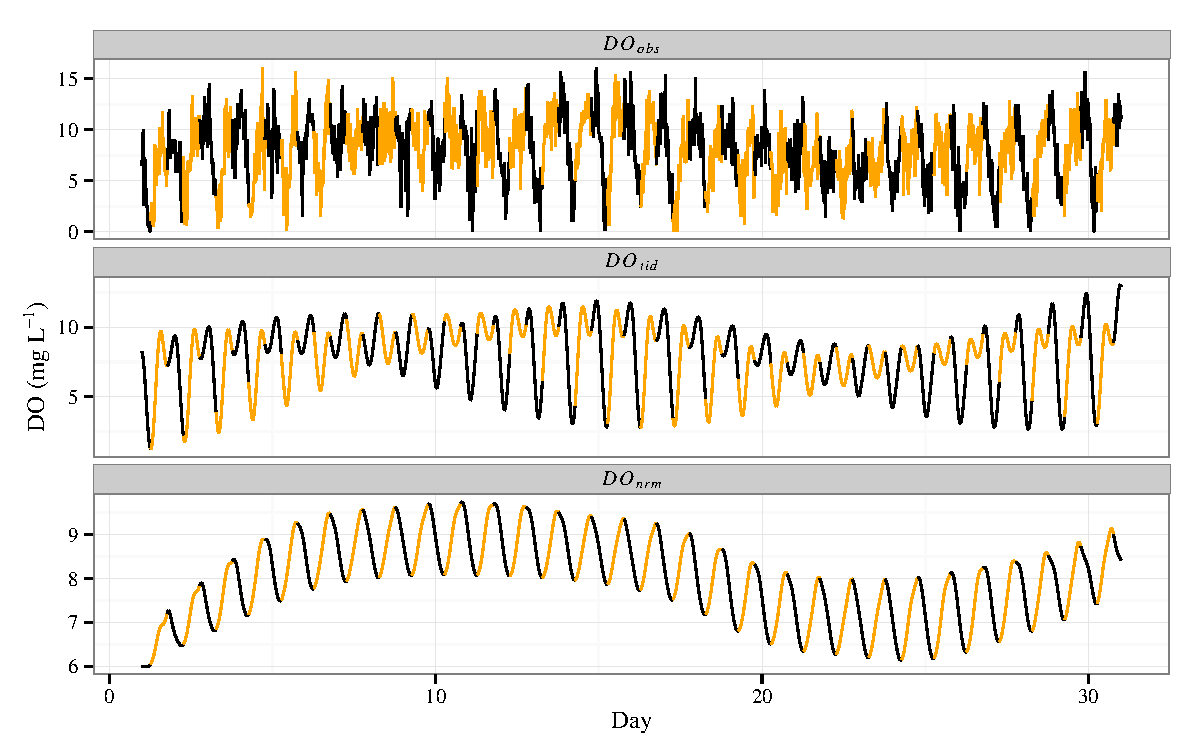
\includegraphics[width=\maxwidth]{figure/do_dtd} 

}

\caption[Example of detiding a simulated \ac{DO} time series]{Example of detiding a simulated \ac{DO} time series.  Simulated values are those in \cref{fig:do_sim}.  Yellow indicates daylight periods.\label{fig:do_dtd}}
\end{figure}


\end{knitrout}
\vfill
\clearpage

% example of creating simulated time series
\centering\vspace*{\fill}
\begin{knitrout}
\definecolor{shadecolor}{rgb}{0.969, 0.969, 0.969}\color{fgcolor}\begin{figure}[!ht]


{\centering 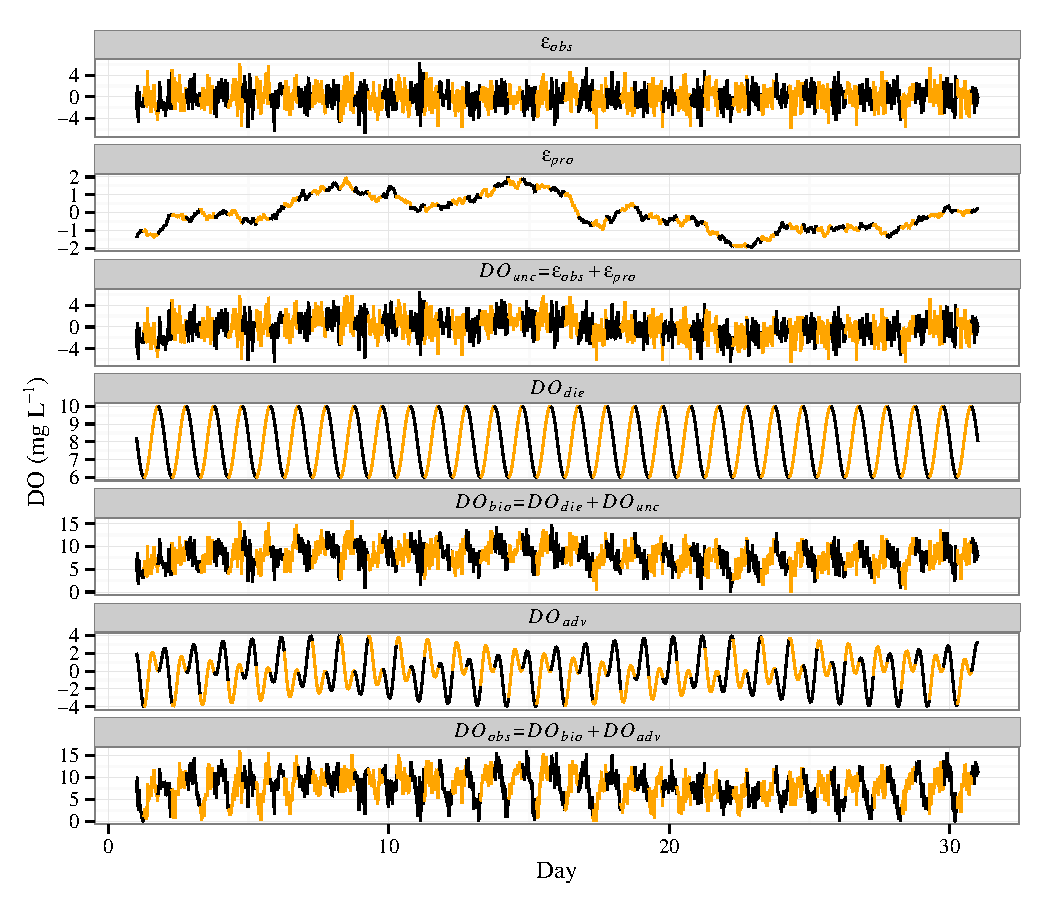
\includegraphics[width=\maxwidth]{figure/do_sim} 

}

\caption[Example of creating a simulated \ac{DO} time series]{Example of creating a simulated \ac{DO} time series.  Values were simulated every 30 minutes for 30 days.  Yellow indicates daylight periods.\label{fig:do_sim}}
\end{figure}


\end{knitrout}
\vfill
\clearpage

% plot of representative time series for simulation
\centering\vspace*{\fill}
\begin{knitrout}
\definecolor{shadecolor}{rgb}{0.969, 0.969, 0.969}\color{fgcolor}\begin{figure}[!ht]


{\centering 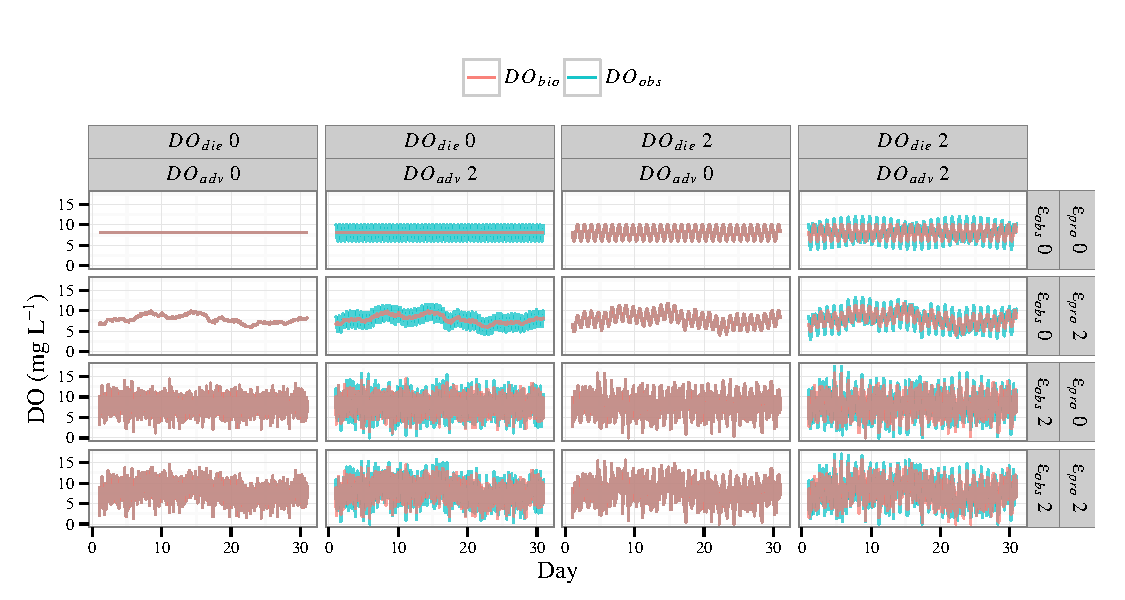
\includegraphics[width=\maxwidth]{figure/sim_ex} 

}

\caption[Representative examples of simulated \ac{DO} time series created by varying each of five parameters]{Representative examples of simulated \ac{DO} time series created by varying each of five parameters: tidal category (e.g., Mixed), strength of tidal association with \ac{DO} signal using $DO_{adv}$, amount of process uncertainty $\epsilon_{pro}$, amount of observation observation uncertainty $\epsilon_{obs}$, and strength of diel \ac{DO} component $DO_{die}$.  Parameter values represent the extremes used in the simulation (i.e., minimum, maximum).  Black lines are observed \ac{DO} from \cref{do_obs_all} and red lines are biological \ac{DO} from \cref{do_bio}.\label{fig:sim_ex}}
\end{figure}


\end{knitrout}
\vfill
\clearpage

% example of error surfaces 
\centering\vspace*{\fill}
\begin{knitrout}
\definecolor{shadecolor}{rgb}{0.969, 0.969, 0.969}\color{fgcolor}\begin{figure}[!ht]


{\centering 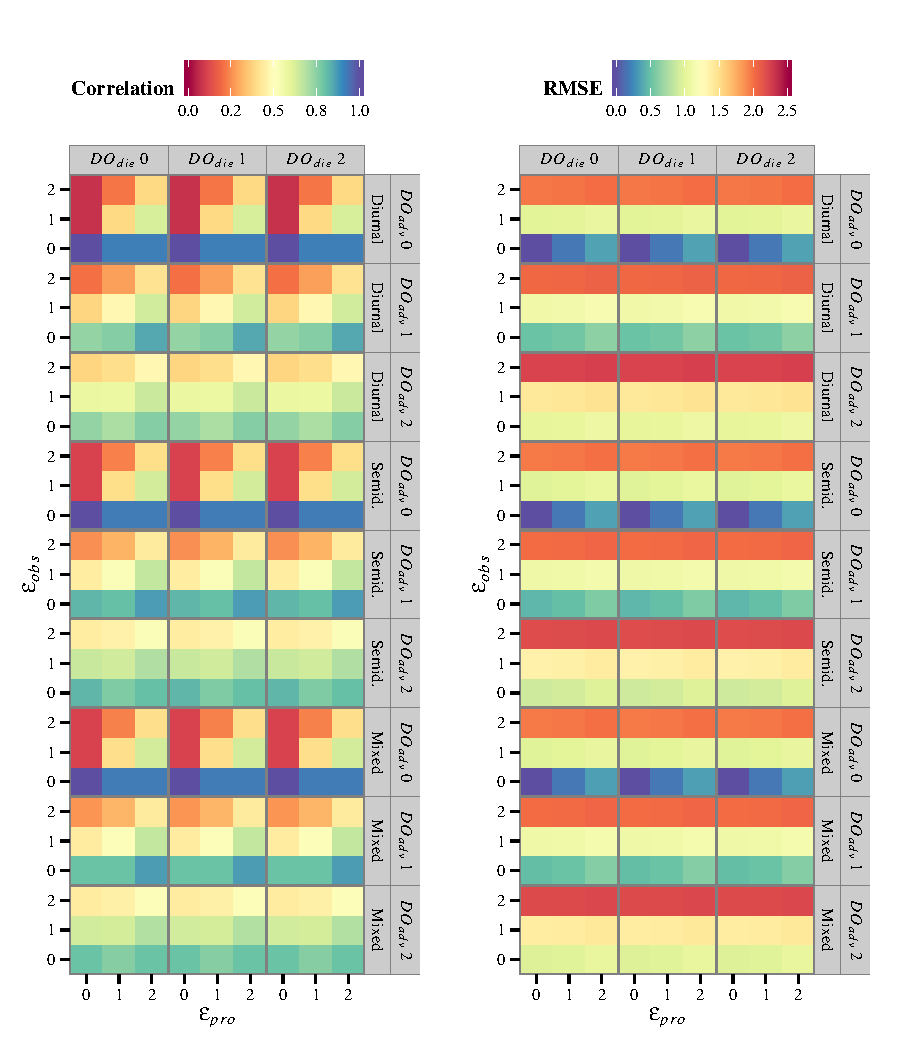
\includegraphics[width=\maxwidth]{figure/err_surf1} 

}

\caption[Correlations and errors (\ac{RMSE}) for detided \ac{DO} time series, $DO_{dtd}$, from weighted regression with `true' biological \ac{DO}, $DO_{bio}$, for varying simulation parameters]{Correlations and errors (\ac{RMSE}) for detided \ac{DO} time series, $DO_{dtd}$, from weighted regression with `true' biological \ac{DO}, $DO_{bio}$, for varying simulation parameters: tidal category (e.g., Mixed), strength of tidal association with \ac{DO} signal $DO_{adv}$, amount of process uncertainty $\epsilon_{pro}$, amount of observation observation uncertainty $\epsilon_{obs}$, and strength of diel \ac{DO} component $DO_{die}$.  Each tile represents the correlation or error between detided and biological \ac{DO} time series from results for a given combination of simulation parameters.  Results are averaged for all window widths used to evaluate the regressions.\label{fig:err_surf1}}
\end{figure}


\end{knitrout}
\vfill
\clearpage

% example of error surfaces 
\centering\vspace*{\fill}
\begin{knitrout}
\definecolor{shadecolor}{rgb}{0.969, 0.969, 0.969}\color{fgcolor}\begin{figure}[!ht]


{\centering 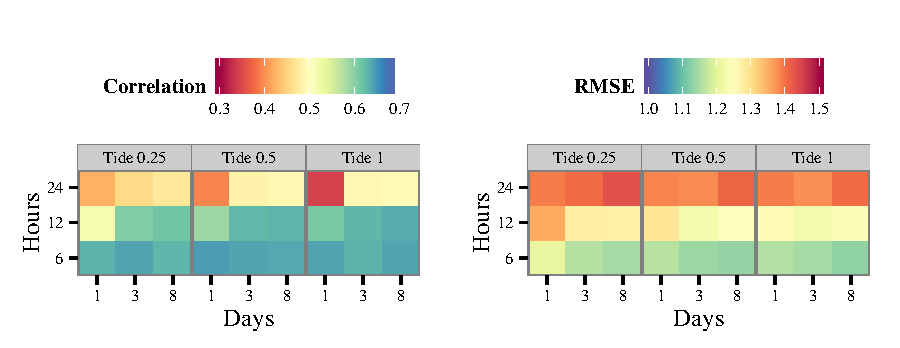
\includegraphics[width=\maxwidth]{figure/err_surf2} 

}

\caption[Correlations and errors (\ac{RMSE}) for detided \ac{DO} time series, $DO_{dtd}$, from weighted regression with `true' biological \ac{DO}, $DO_{bio}$, for varying half window widths]{Correlations and errors (\ac{RMSE}) for detided \ac{DO} time series, $DO_{dtd}$, from weighted regression with `true' biological \ac{DO}, $DO_{bio}$, for varying half window widths: days, hour of day, and proportion of tidal range.  Each tile represents the correlation or error between detided and biological \ac{DO} time series from results for a given combination of window widths.  Results are averaged for all simulation parameters used to evaluate the regressions.\label{fig:err_surf2}}
\end{figure}


\end{knitrout}
\vfill
\clearpage

% maps of each case
\centering\vspace*{\fill}
\begin{knitrout}
\definecolor{shadecolor}{rgb}{0.969, 0.969, 0.969}\color{fgcolor}\begin{figure}[!ht]


{\centering 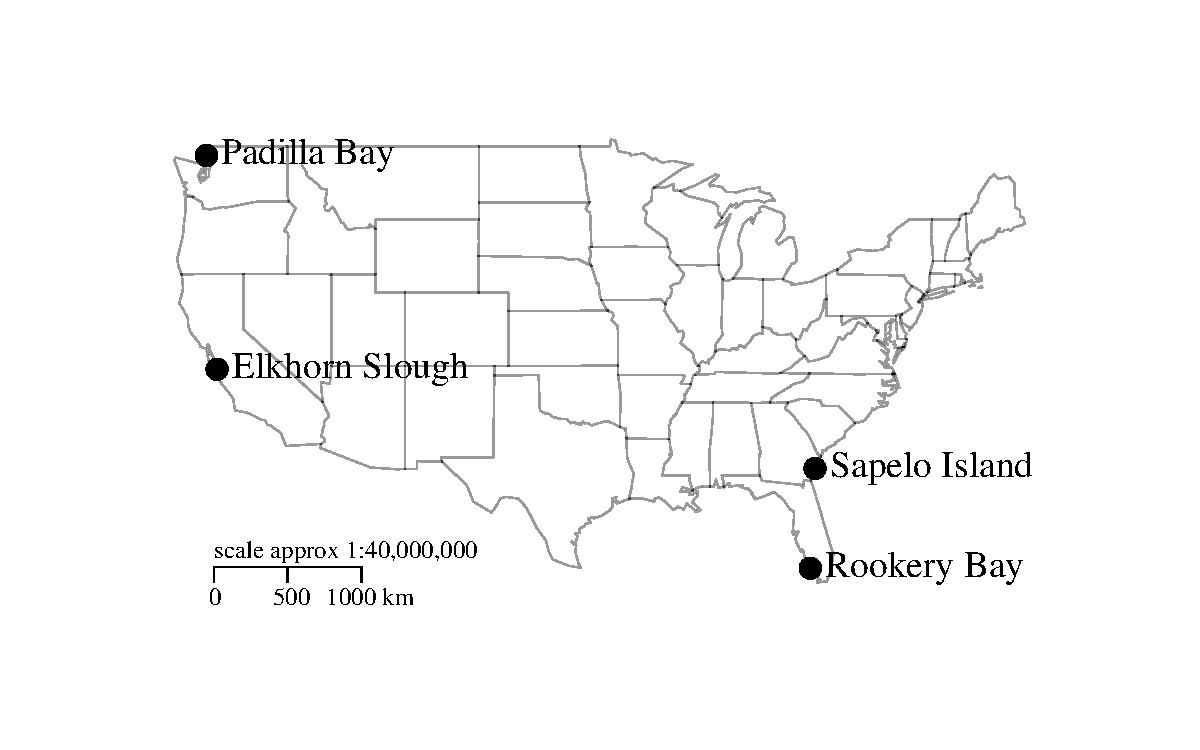
\includegraphics[width=\maxwidth]{figure/case_map} 

}

\caption[Locations of \ac{NERRS} sites used as case studies to evaluate of weighted regression]{Locations of \ac{NERRS} sites used as case studies to evaluate of weighted regression.  Individual stations at each reserve are PDBJE (Joe Leary Estuary at Padilla Bay), RKBMB (Middle Blackwater River at Rookery Bay), SAPDC (Dean Creek at Sapelo Island), and TJRBR (Boca Rio at Tijuana River).\label{fig:case_map}}
\end{figure}


\end{knitrout}
\vfill
\clearpage

% example from RKBMB
\centering\vspace*{\fill}
\begin{knitrout}
\definecolor{shadecolor}{rgb}{0.969, 0.969, 0.969}\color{fgcolor}\begin{figure}[!ht]


{\centering 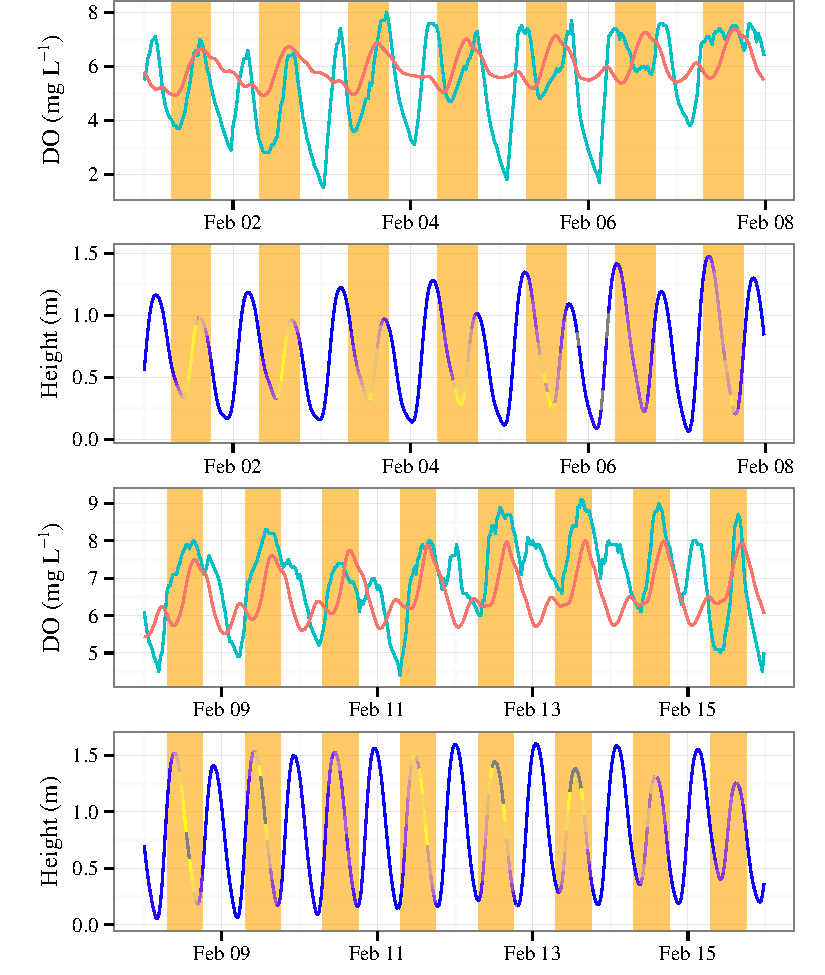
\includegraphics[width=0.8\textwidth]{figure/case_ex1} 

}

\caption[Example of daily mean metabolism (top) and continuous \ac{DO} time series (middle) before (observed) and after (detided) detiding with weighted regression]{Example of daily mean metabolism (top) and continuous \ac{DO} time series (middle) before (observed) and after (detided) detiding with weighted regression. Tidal height colored by total photosynthetically active radiation (mmol m$^{-2}$) is on the bottom plot. Results are for the Rookery Bay station for twenty days in July, 2012 using a weighted regression with window of eight days, six hours within each day, and tidal height proportion of one.\label{fig:case_ex1}}
\end{figure}


\end{knitrout}
\vfill
\clearpage

% example from SAPDC
\centering\vspace*{\fill}
\begin{knitrout}
\definecolor{shadecolor}{rgb}{0.969, 0.969, 0.969}\color{fgcolor}\begin{figure}[!ht]


{\centering 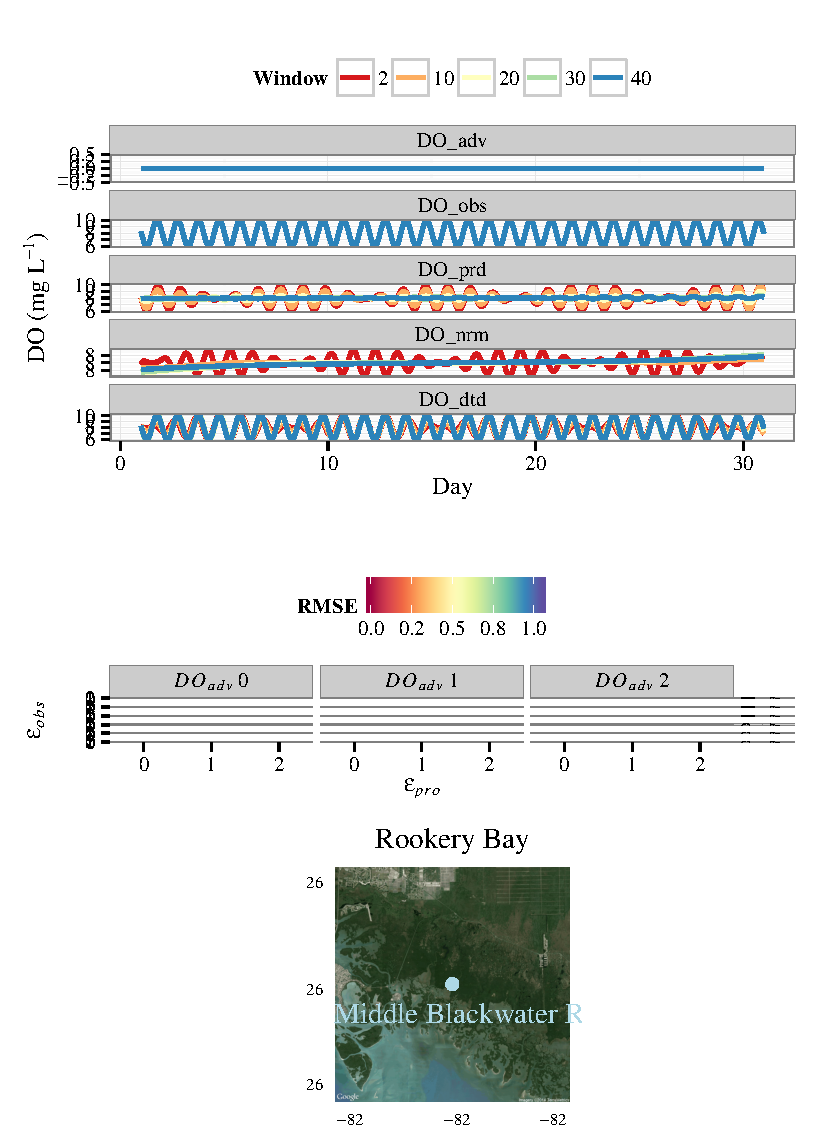
\includegraphics[width=0.8\textwidth]{figure/case_ex2} 

}

\caption[Example of daily mean metabolism (top) and continuous \ac{DO} time series (middle) before (observed) and after (detided) detiding with weighted regression]{Example of daily mean metabolism (top) and continuous \ac{DO} time series (middle) before (observed) and after (detided) detiding with weighted regression. Tidal height colored by total photosynthetically active radiation (mmol m$^{-2}$) is on the bottom plot. Results are for the Sapelo Island station for a twenty day period in February, 2012 using weighted regression with a window of eight days, six hours within each day, and tidal height proportion of one.\label{fig:case_ex2}}
\end{figure}


\end{knitrout}

% plots of summarized metabolism estimates, before/after detiding
% ELKVM, PDBBY
\centering\vspace*{\fill}
\begin{knitrout}
\definecolor{shadecolor}{rgb}{0.969, 0.969, 0.969}\color{fgcolor}\begin{figure}[!ht]


{\centering 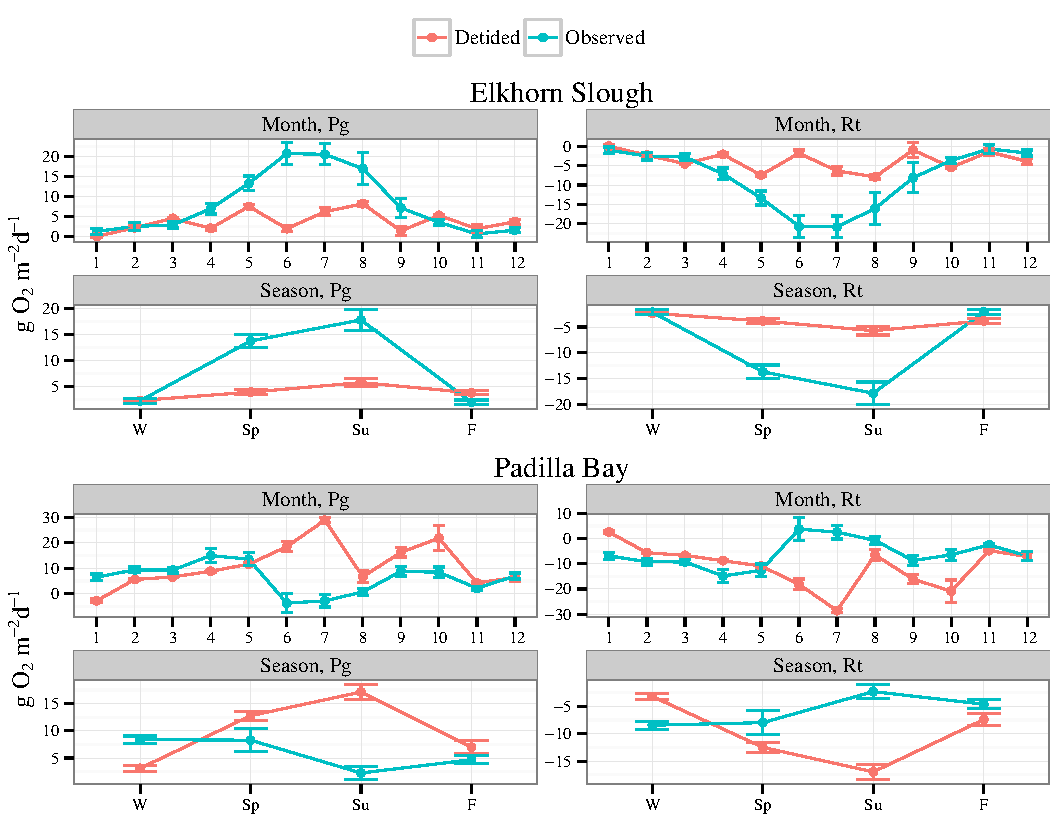
\includegraphics[width=\maxwidth]{figure/metab_sum1} 

}

\caption[Means and standard errors of daily metabolism estimates (gross production, total respiration, net ecosystem metabolism) aggregated by month and season]{Means and standard errors of daily metabolism estimates (gross production, total respiration, net ecosystem metabolism) aggregated by month and season.  Aggregated estimates are for Elkhorn Slough and Padilla Bay from observed and detided \ac{DO} time series.\label{fig:metab_sum1}}
\end{figure}


\end{knitrout}
\vfill
\clearpage

% RKBMB, SAPDC
% plots of summarized metabolism estimates, before/after detiding
\centering\vspace*{\fill}
\begin{knitrout}
\definecolor{shadecolor}{rgb}{0.969, 0.969, 0.969}\color{fgcolor}\begin{figure}[!ht]


{\centering 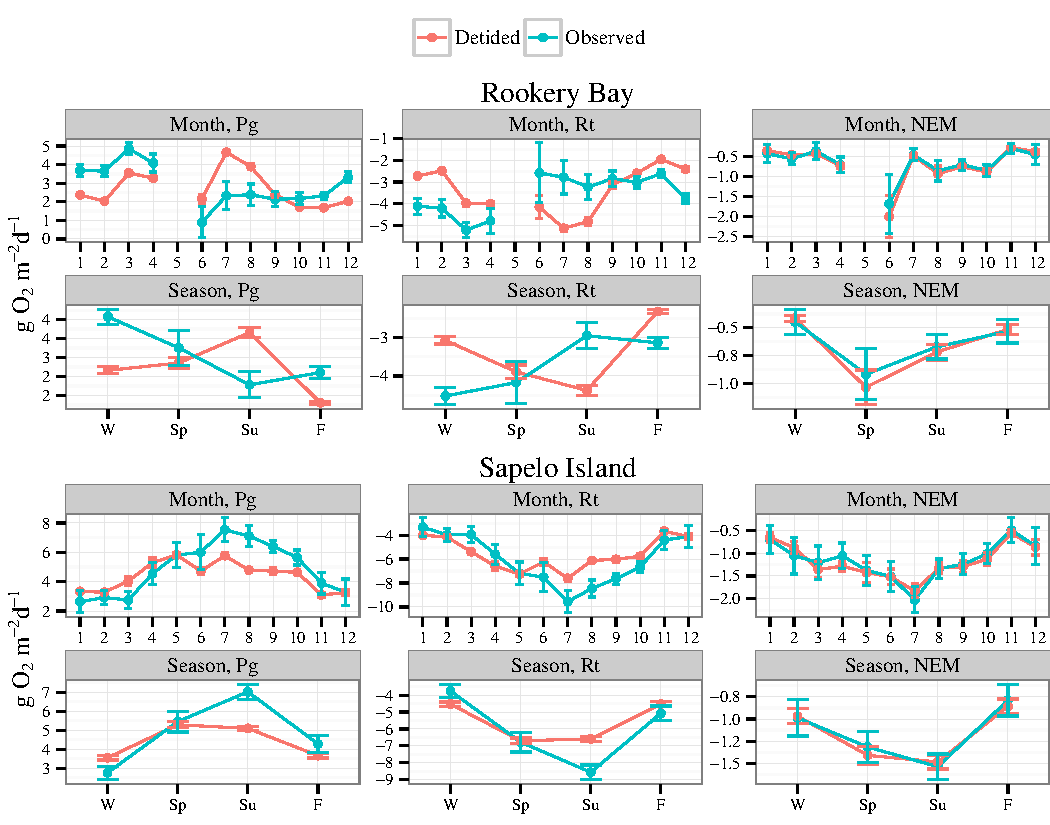
\includegraphics[width=\maxwidth]{figure/metab_sum2} 

}

\caption[Means and standard errors of daily metabolism estimates (gross production, total respiration, net ecosystem metabolism) aggregated by month and season]{Means and standard errors of daily metabolism estimates (gross production, total respiration, net ecosystem metabolism) aggregated by month and season.  Aggregated estimates are for Rookery Bay and Sapelo Island from observed and detided \ac{DO} time series.  May was removed from Rookery Bay because of incomplete data.\label{fig:metab_sum2}}
\end{figure}


\end{knitrout}
\vfill
\clearpage

%%%%%%
% tables

\section{Tables}

% summary of simulation performance for detided and biological, sim parameters
% latex.default(tab, file = "", where = "h", rowlabel = "Parameter",      caption = cap.val, caption.loc = "top", rgroup = Parms, n.rgroup = rep(3,          5), cgroup = c("Correlation", "RMSE"), n.cgroup = c(5,          5), rowname = rows, colheads = rep(c("Min", "25\\textsuperscript{th}",          "Mean", "75\\textsuperscript{th}", "Max"), 2), label = "tab:dtd_perf1") 
%
\begin{table}[h]
\caption{Summary (range, mean, percentiles) of correlations and error estimates comparing detided and biological \ac{DO} time series for different simulation parameters (tidal category, $DO_{die}$, $DO_{adv}$, $\epsilon_{pro}$, $\epsilon_{obs}$).  Values represent a combination of results from multiple simulations with the parameter value held constant for each row (e.g., row one is a summary of all simulations for which the tidal category was diurnal).\label{tab:dtd_perf1}} 
\begin{center}
\begin{tabular}{llllllclllll}
\hline\hline
\multicolumn{1}{l}{\bfseries Parameter}&\multicolumn{5}{c}{\bfseries Correlation}&\multicolumn{1}{c}{\bfseries }&\multicolumn{5}{c}{\bfseries RMSE}\tabularnewline
\cline{2-6} \cline{8-12}
\multicolumn{1}{l}{}&\multicolumn{1}{c}{Min}&\multicolumn{1}{c}{25\textsuperscript{th}}&\multicolumn{1}{c}{Mean}&\multicolumn{1}{c}{75\textsuperscript{th}}&\multicolumn{1}{c}{Max}&\multicolumn{1}{c}{}&\multicolumn{1}{c}{Min}&\multicolumn{1}{c}{25\textsuperscript{th}}&\multicolumn{1}{c}{Mean}&\multicolumn{1}{c}{75\textsuperscript{th}}&\multicolumn{1}{c}{Max}\tabularnewline
\hline
{\bfseries Tidal category}&&&&&&&&&&&\tabularnewline
~~Diurnal&-0.78&0.35&0.54&0.80&1.00&&0.00&0.86&1.29&1.99&2.39\tabularnewline
~~Semidiurnal&-0.28&0.37&0.58&0.84&1.00&&0.00&0.73&1.25&1.97&2.40\tabularnewline
~~Mixed Semidiurnal&-0.39&0.37&0.57&0.83&1.00&&0.00&0.78&1.27&1.97&2.47\tabularnewline
\hline
{\bfseries $\boldsymbol{DO_{die}}$}&&&&&&&&&&&\tabularnewline
~~0& 0.00&0.21&0.52&0.92&1.00&&0.00&0.26&1.05&1.96&2.05\tabularnewline
~~1&-0.78&0.36&0.55&0.74&1.00&&0.12&0.68&1.23&2.00&2.13\tabularnewline
~~2&-0.78&0.48&0.62&0.81&1.00&&0.25&1.13&1.53&2.08&2.47\tabularnewline
\hline
{\bfseries $\boldsymbol{DO_{adv}}$}&&&&&&&&&&&\tabularnewline
~~0&-0.78&0.36&0.56&0.82&1.00&&0.00&0.78&1.27&1.98&2.47\tabularnewline
~~1&-0.78&0.36&0.56&0.82&1.00&&0.00&0.78&1.27&1.98&2.47\tabularnewline
~~2&-0.78&0.36&0.56&0.82&1.00&&0.00&0.78&1.27&1.98&2.47\tabularnewline
\hline
{\bfseries $\boldsymbol{\epsilon_{pro}}$}&&&&&&&&&&&\tabularnewline
~~0&-0.78&0.14&0.50&0.83&1.00&&0.00&0.74&1.23&1.96&2.45\tabularnewline
~~1& 0.14&0.35&0.55&0.81&0.99&&0.07&0.76&1.26&1.98&2.45\tabularnewline
~~2& 0.33&0.47&0.65&0.82&0.99&&0.15&0.82&1.32&2.00&2.47\tabularnewline
\hline
{\bfseries $\boldsymbol{\epsilon_{obs}}$}&&&&&&&&&&&\tabularnewline
~~0&-0.78&0.80&0.84&0.97&1.00&&0.00&0.26&0.57&0.78&1.57\tabularnewline
~~1&-0.07&0.39&0.51&0.67&0.84&&0.96&1.01&1.18&1.25&1.82\tabularnewline
~~2& 0.00&0.22&0.34&0.44&0.63&&1.93&1.98&2.07&2.11&2.47\tabularnewline
\hline
\end{tabular}
\end{center}
\end{table}



% summary of simulation performance for detided and biological, window widths
% latex.default(tab, file = "", rowlabel = "Window", caption = cap.val,      caption.loc = "top", rgroup = Parms, n.rgroup = rep(3, 3),      cgroup = c("Correlation", "RMSE"), n.cgroup = c(5, 5), rowname = rows,      colheads = rep(c("Min", "25\\textsuperscript{th}", "Mean",          "75\\textsuperscript{th}", "Max"), 2), label = "tab:dtd_perf2") 
%
\begin{table}[!tbp]
\caption{Summary (range, mean, percentiles) of correlations and error estimates comparing detided and biological \ac{DO} time series for simulations using different half window widths in the weighted regressions (days, hours, and proportion of tidal range).  Values represent a combination of results from multiple simulations with the window value held constant for each row (e.g., row one is a summary of all simulations for which the half window width was one day).\label{tab:dtd_perf2}} 
\begin{center}
\begin{tabular}{llllllclllll}
\hline\hline
\multicolumn{1}{l}{\bfseries Window}&\multicolumn{5}{c}{\bfseries Correlation}&\multicolumn{1}{c}{\bfseries }&\multicolumn{5}{c}{\bfseries RMSE}\tabularnewline
\cline{2-6} \cline{8-12}
\multicolumn{1}{l}{}&\multicolumn{1}{c}{Min}&\multicolumn{1}{c}{25\textsuperscript{th}}&\multicolumn{1}{c}{Mean}&\multicolumn{1}{c}{75\textsuperscript{th}}&\multicolumn{1}{c}{Max}&\multicolumn{1}{c}{}&\multicolumn{1}{c}{Min}&\multicolumn{1}{c}{25\textsuperscript{th}}&\multicolumn{1}{c}{Mean}&\multicolumn{1}{c}{75\textsuperscript{th}}&\multicolumn{1}{c}{Max}\tabularnewline
\hline
{\bfseries Days}&&&&&&&&&&&\tabularnewline
~~1&-0.78&0.30&0.53&0.77&1.00&&0.00&0.95&1.29&1.96&2.40\tabularnewline
~~3& 0.00&0.39&0.58&0.83&1.00&&0.00&0.75&1.26&1.98&2.43\tabularnewline
~~8& 0.03&0.36&0.58&0.85&1.00&&0.00&0.78&1.27&1.99&2.47\tabularnewline
\hline
{\bfseries Hours}&&&&&&&&&&&\tabularnewline
~~6& 0.00&0.41&0.64&0.90&1.00&&0.00&0.53&1.15&1.97&2.21\tabularnewline
~~12& 0.04&0.41&0.61&0.85&1.00&&0.00&0.87&1.27&1.98&2.33\tabularnewline
~~24&-0.78&0.24&0.45&0.60&1.00&&0.00&0.98&1.40&1.98&2.47\tabularnewline
\hline
{\bfseries Tide}&&&&&&&&&&&\tabularnewline
~~0.25& 0.03&0.35&0.55&0.81&1.00&&0.00&0.81&1.29&1.99&2.47\tabularnewline
~~0.5&-0.10&0.37&0.57&0.82&1.00&&0.00&0.78&1.26&1.97&2.40\tabularnewline
~~1&-0.78&0.36&0.57&0.82&1.00&&0.00&0.76&1.26&1.97&2.40\tabularnewline
\hline
\end{tabular}
\end{center}
\end{table}



% descriptive table of case studies
% latex.default(tab, file = "", rowlabel = "Site", insert.bottom = foot.val,      caption = cap.val, caption.loc = "top", cgroup = c("Tidal amplitude",          "DO", "Metabolism\\textsuperscript{\\textit{a}}"), n.cgroup = c(4,          2, 3), rowname = rows, colheads = c("O1", "P1", "M2",          "S2", "Range", "Mean", "Pg", "Rt", "NEM"), label = "tab:case_att") 
%
\begin{table}[!tbp]
\caption{Summary statistics of tidal component amplitudes (m), \ac{DO} (mg L$^{-1}$), and metabolism estimates (gross production, respiration, and net ecosystem metabolism as g m$^{-2}$ d$^{-1}$) for each case study.  Tidal components are principal lunar semidiurnal (O1, frequency 25.82 hours), solar diurnal (P1, 24.07 hours), lunar semidiurnal (M2, 12.42 hours), and solar semidiurnal (S2, 12 hours), estimated from harmonic regressions of tidal height (\texttt{oce} package in R, \citealt{Foreman89}, \citetalias{RDCT14}).  \ac{DO} range and mean are grand means of daily estimates for the entire period of record (30 minute observations) for each site.  Metabolism estimates are means of daily integrated values.\label{tab:case_att}} 
\begin{center}
\begin{tabular}{lllllcllclll}
\hline\hline
\multicolumn{1}{l}{\bfseries Site}&\multicolumn{4}{c}{\bfseries Tidal amplitude}&\multicolumn{1}{c}{\bfseries }&\multicolumn{2}{c}{\bfseries DO}&\multicolumn{1}{c}{\bfseries }&\multicolumn{3}{c}{\bfseries Metabolism\textsuperscript{\textit{a}}}\tabularnewline
\cline{2-5} \cline{7-8} \cline{10-12}
\multicolumn{1}{l}{}&\multicolumn{1}{c}{O1}&\multicolumn{1}{c}{P1}&\multicolumn{1}{c}{M2}&\multicolumn{1}{c}{S2}&\multicolumn{1}{c}{}&\multicolumn{1}{c}{Range}&\multicolumn{1}{c}{Mean}&\multicolumn{1}{c}{}&\multicolumn{1}{c}{Pg}&\multicolumn{1}{c}{Rt}&\multicolumn{1}{c}{NEM}\tabularnewline
\hline
ELKVM&0.24&0.12&0.48&0.13&&6.79&7.86&&8.14&-8.19&-0.05\tabularnewline
PDBBY&0.46&0.23&0.63&0.15&&7.53&8.97&&5.95&-5.90& 0.05\tabularnewline
RKBMB&0.13&0.04&0.36&0.10&&5.47&4.53&&3.02&-3.62&-0.60\tabularnewline
SAPDC&0.10&0.02&0.54&0.07&&7.98&5.01&&4.89&-6.04&-1.16\tabularnewline
\hline
\end{tabular}
\end{center}
\footnotesize\textsuperscript{\textit{a}}Pg: gross production, Rt: respiration, NEM: net ecosystem metabolism\end{table}



% correlations with tide before/after wtreg
% latex.default(tab, file = "", rowlabel = "Site", rgroup = unique(rows),      n.rgroup = rep(2, 4), insert.bottom = foot.val, caption = cap.val,      colheads = c("DO", "Pg\\textsuperscript{\\textit{a}}", "Rt",          "NEM"), caption.loc = "top", rowname = rep(c("Observed",          "Detided"), 4), label = "tab:cor_res") 
%
\begin{table}[!tbp]
\caption{Correlations of tidal changes at each site with continuous \ac{DO} observations and metabolism estimates (gross production, respiration, and net metabolism) before (observed) and after (detided) detiding from weighted regression.  \ac{DO} values are correlated with predicted tidal height at each observation, whereas metabolism estimates are correlated with mean tidal height change between observations during day, night, or total day periods for production, respiration, and net metabolism, respectively.\label{tab:cor_res}} 
\begin{center}
\begin{tabular}{lllll}
\hline\hline
\multicolumn{1}{l}{Site}&\multicolumn{1}{c}{DO}&\multicolumn{1}{c}{Pg\textsuperscript{\textit{a}}}&\multicolumn{1}{c}{Rt}&\multicolumn{1}{c}{NEM}\tabularnewline
\hline
{\bfseries ELKVM}&&&&\tabularnewline
~~Observed& 0.47***& 0.60***& 0.73***& 0.35***\tabularnewline
~~Detided&-0.02*&-0.04 &-0.17**& 0.06 \tabularnewline
\hline
{\bfseries PDBBY}&&&&\tabularnewline
~~Observed&-0.45***&-0.33***&-0.46***&-0.25***\tabularnewline
~~Detided& 0.09***& 0.57***& 0.51***&-0.12*\tabularnewline
\hline
{\bfseries RKBMB}&&&&\tabularnewline
~~Observed& 0.28***& 0.34***& 0.39***& 0.24***\tabularnewline
~~Detided&-0.02*&-0.36***&-0.44***& 0.11 \tabularnewline
\hline
{\bfseries SAPDC}&&&&\tabularnewline
~~Observed& 0.48***& 0.54***& 0.71***& 0.41***\tabularnewline
~~Detided&-0.03***& 0.08 & 0.15**&-0.06 \tabularnewline
\hline
\end{tabular}
\end{center}
\footnotesize *$p<0.05$; **$p<0.01$; ***$p<0.001$\\\textsuperscript{\textit{a}}Pg: gross production, Rt: respiration, NEM: net ecosystem metabolism\end{table}



% case study metabolism results, including perc anom
% latex.default(tab, file = "", rowlabel = "Site", insert.bottom = foot.val,      caption = cap.val, caption.loc = "top", rgroup = unique(to_tab$Site),      n.rgroup = rep(2, 4), cgroup = c("Pg\\textsuperscript{\\textit{a}}",          "Rt", "NEM"), n.cgroup = c(3, 3, 2), rowname = rows,      colheads = c(rep(c("Mean", "Std. Err.", "Anom"), 2), c("Mean",          "Std. Err.")), label = "tab:case_res") 
%
\begin{table}[!tbp]
\caption{Summary of metabolism estimates (gross production, respiration, and net metabolism) for case studies using \ac{DO} time series before (observed) and after (detided) application of weighted regression.  Means and standard errors are based on daily integrated metabolism estimates.  Anomalous values are the proportion of metabolism estimates that were negative for gross production and positive for respiration.  Results are for weighted regressions with a window of thirty days and tidal height proportion of one.\label{tab:case_res}} 
\begin{center}
\begin{tabular}{llllclllcll}
\hline\hline
\multicolumn{1}{l}{\bfseries Site}&\multicolumn{3}{c}{\bfseries Pg\textsuperscript{\textit{a}}}&\multicolumn{1}{c}{\bfseries }&\multicolumn{3}{c}{\bfseries Rt}&\multicolumn{1}{c}{\bfseries }&\multicolumn{2}{c}{\bfseries NEM}\tabularnewline
\cline{2-4} \cline{6-8} \cline{10-11}
\multicolumn{1}{l}{}&\multicolumn{1}{c}{Mean}&\multicolumn{1}{c}{Std. Err.}&\multicolumn{1}{c}{Anom}&\multicolumn{1}{c}{}&\multicolumn{1}{c}{Mean}&\multicolumn{1}{c}{Std. Err.}&\multicolumn{1}{c}{Anom}&\multicolumn{1}{c}{}&\multicolumn{1}{c}{Mean}&\multicolumn{1}{c}{Std. Err.}\tabularnewline
\hline
{\bfseries ELKVM}&&&&&&&&&&\tabularnewline
~~Observed&8.14&0.67&0.19&&-8.19&0.69&0.21&&-0.05&0.16\tabularnewline
~~Detided&2.78&0.14&0.11&&-2.83&0.15&0.12&&-0.05&0.03\tabularnewline
\hline
{\bfseries PDBBY}&&&&&&&&&&\tabularnewline
~~Observed&5.95&0.69&0.22&&-5.90&0.74&0.19&& 0.05&0.22\tabularnewline
~~Detided&8.07&0.40&0.05&&-8.04&0.39&0.06&& 0.04&0.06\tabularnewline
\hline
{\bfseries RKBMB}&&&&&&&&&&\tabularnewline
~~Observed&3.02&0.14&0.09&&-3.62&0.15&0.08&&-0.60&0.06\tabularnewline
~~Detided&2.73&0.07&0.00&&-3.34&0.07&0.00&&-0.61&0.03\tabularnewline
\hline
{\bfseries SAPDC}&&&&&&&&&&\tabularnewline
~~Observed&4.89&0.23&0.13&&-6.04&0.25&0.11&&-1.16&0.09\tabularnewline
~~Detided&4.40&0.08&0.00&&-5.58&0.09&0.00&&-1.18&0.05\tabularnewline
\hline
\end{tabular}
\end{center}
\textsuperscript{\textit{a}}Pg: gross production, Rt: respiration, NEM: net ecosystem metabolism\end{table}



\end{document}
